\documentclass[11pt,a4paper,reqno]{amsart}

\usepackage[utf8]{inputenc}
\usepackage[T1]{fontenc}
\usepackage{lmodern}
\usepackage{amsmath,amssymb,amsthm,mathtools}
\usepackage{booktabs}
\usepackage{array}
\usepackage{graphicx}
\usepackage{xcolor}
\definecolor{acadblue}{rgb}{0.0, 0.24, 0.52}
\usepackage[margin=2.45cm]{geometry}
\usepackage[colorlinks=true,linkcolor=acadblue,citecolor=acadblue,urlcolor=acadblue]{hyperref}

\newtheorem{theorem}{Theorem}[section]
\newtheorem{proposition}[theorem]{Proposition}
\newtheorem{lemma}[theorem]{Lemma}
\newtheorem{corollary}[theorem]{Corollary}
\theoremstyle{definition}
\newtheorem{definition}[theorem]{Definition}
\theoremstyle{remark}
\newtheorem{remark}[theorem]{Remark}

\numberwithin{equation}{section}
\allowdisplaybreaks
\emergencystretch=1.5em

\newcommand{\dd}{\mathrm{d}}
\newcommand{\ii}{\mathrm{i}}
\newcommand{\ee}{\mathrm{e}}
\newcommand{\Rea}{\operatorname{Re}}
\newcommand{\Ima}{\operatorname{Im}}
\newcommand{\Wig}{\mathcal{W}}
\newcommand{\Wtil}{\widetilde{W}}
\newcommand{\fac}{\mathclose{\mathchar"0021}}

\title[Wigner Phase-Space and Shifted Contours for Riemann's $\Xi$-Function]{Wigner Phase-Space Representation, Shifted Cauchy Contours, and Local Saddle-Point Coalescence in the Transverse Wronskian of Riemann's $\Xi$-Function}

\author{Thijs Missiaen}
\address{Independent Researcher, Belgium (ORCID: 0009-0007-3678-0810)}
\email{thijs.missiaen@gmail.com}
\urladdr{https://orcid.org/0009-0007-3678-0810}

\subjclass[2020]{Primary 11M06, 30E15; Secondary 81S30, 42B10, 65D30}
\keywords{Riemann Xi-function, Jacobi theta kernel, transverse Wronskian, Wigner phase-space distribution, Hudson theorem, Cauchy contour conditioning, local saddle-point coalescence}

\date{November 2026}

\begin{document}

\begin{abstract}
We study the phase-space and complex-contour structure of the transverse Wronskian $W(d,t) = \frac{1}{2}\partial_d|\Xi(t-\ii d)|^2$ of Riemann's completed zeta function $\Xi(t-\ii d) = \xi(\frac{1}{2}+d+\ii t)$. First, we express $W(d,t) = 16\int_0^\infty y\sinh(2d y)\,I(y,t)\,\dd y$ in terms of the canonical Wigner distribution $I(y,t) = 2\pi\Wig_\Phi(y/2, 2t)$ of the Jacobi--Riemann kernel $\Phi(u)$ and show via Hudson's theorem and the zero-marginal identity $\int_0^\infty I(y,\gamma_k)\,\dd y = 0$ that $I(y,t)$ changes sign. Second, we prove holomorphic parity $\Phi(-u)=\Phi(u)$ on $|\Ima(u)| < \pi/8$ and double-exponential vertical-wall decay on $|\Ima(z)| < \pi/4$, showing that horizontal contour shifts preserve $I(y,t)$ by Cauchy's theorem while improving $L^1$ quadrature conditioning. Third, we derive the local pitchfork normal form for stationary points of $\ln G_y(z) + 2\ii t z$ away from zeros of $\Phi(u)$, locate explicit zeros of $\Phi(u)$ inside $|\Ima(u)| < \pi/8$, and document why this formalism applies equally to functions with off-critical zeros.
\end{abstract}

\maketitle

\section{Introduction}\label{sec:intro}

Let $\xi(s) = \frac{1}{2}s(s-1)\pi^{-s/2}\Gamma(s/2)\zeta(s)$ denote Riemann's completed zeta function, and set $s = \frac{1}{2} + d + \ii t$ with transverse offset $d = \sigma - \frac{1}{2} \in \mathbb{R}$ and spectral height $t \in \mathbb{R}$. Writing $z = -\ii(s - \frac{1}{2}) = t - \ii d$, Riemann's entire function $\Xi(z) := \xi(\frac{1}{2} + \ii z) = R(d,t) + \ii I_{\mathrm{im}}(d,t)$ admits the classical Fourier--Laplace representation \cite{Riemann1859,Polya1926,Titchmarsh1986}
\begin{equation}\label{eq:Xi_integral}
\Xi(t - \ii d) = 8\int_0^\infty \Phi(u)\cos\bigl(2(t - \ii d)u\bigr)\,\dd u = 4\int_{-\infty}^\infty \Phi(u)\,\ee^{2(d + \ii t)u}\,\dd u,
\end{equation}
where the rapidly decaying kernel $\Phi(u)$ is generated by the Jacobi theta series $\theta(w) = \sum_{n\in\mathbb{Z}} \ee^{-\pi n^2 w}$ ($\Rea w > 0$) via
\begin{equation}\label{eq:Phi_def}
\Phi(u) := \sum_{n=1}^\infty \phi_n(u), \qquad \phi_n(u) := \left(2\pi^2 n^4 \ee^{9u} - 3\pi n^2 \ee^{5u}\right)\exp\!\left(-\pi n^2 \ee^{4u}\right).
\end{equation}
By the function-theoretic positivity criteria of Hinkkanen \cite{Hinkkanen1997} and Lagarias \cite{Lagarias1999} (building on Speiser's geometric criterion for $\zeta'(s)$ \cite{Speiser1934}), the Riemann Hypothesis is equivalent to the non-negativity of $\Rea(\xi'(s)/\xi(s)) = W(d,t)/|\Xi(t-\ii d)|^2$ throughout $d > 0$, where the \emph{transverse Wronskian} is defined by
\begin{equation}\label{eq:W_def}
W(d,t) := \frac{1}{2}\frac{\partial}{\partial d}\big|\Xi(t-\ii d)\big|^2 = R\,\partial_d R + I_{\mathrm{im}}\,\partial_d I_{\mathrm{im}} = R\,\partial_t I_{\mathrm{im}} - I_{\mathrm{im}}\,\partial_t R.
\end{equation}

When \eqref{eq:W_def} is expanded directly as an oscillatory integral along the real axis, numerical quadrature faces severe cancellation: at $t = \gamma_1 \approx 14.13472514$ and shift $y = 0.40$, positive and negative cosine lobes cancel to $99.7697\%$. At the same time, it is essential not to conflate quadrature conditioning with a proof of positivity: by Cauchy's integral theorem, shifting a horizontal contour leaves the holomorphic integral mathematically unchanged, and the exact autocorrelation identity \eqref{eq:W_mirror_thm} holds for any real-even kernel $\Phi$, including kernels whose Fourier transforms possess off-axis zeros (such as Davenport--Heilbronn linear combinations \cite{DavenportHeilbronn1936,Titchmarsh1986} or backward de Bruijn--Newman deformations $H_\lambda$ with $\lambda < 0$ \cite{DeBruijn1950,Newman1976,CsordasNorfolkVarga1986}).

This note separates three layers with explicit hypotheses: (i) unconditional exact identities for the Wigner autocorrelation representation and shifted Cauchy contours in $|\Ima(z)| < \pi/4$; (ii) a conditional local normal form for complex stationary-point coalescence on open subsets free of zeros of $\Phi$, illustrated numerically at $\omega = 2\gamma_1$; and (iii) explicit analytic obstructions inside the strip (zeros of $\Phi(u)$ creating logarithmic branch points in $\ln G_y(z)$, multi-crossing sign oscillations of $I(y,\gamma_k)$ for $k \ge 3$, and non-multiplicative counterexamples).

\begin{theorem}[Canonical Wigner Identity, Shifted Cauchy Contours, and Local Saddle Normal Form]\label{thm:main}
Let $d \in \mathbb{R}$ and $t \in \mathbb{R}$, and define mirror coordinates $x = u + v$, $y = u - v$ with mirror autocorrelation kernel $G_y(x) := \Phi\!\left(\frac{x+y}{2}\right)\Phi\!\left(\frac{x-y}{2}\right)$. Then:
\begin{enumerate}
\item[\textup{(i)}] \textbf{Canonical Wigner representation and zero-marginal law:} Let $\Wig_\psi(q,p) := (2\pi)^{-1}\int_{\mathbb{R}} \psi(q+x/2)\overline{\psi(q-x/2)}\,\ee^{-\ii p x}\,\dd x$ denote the standard quantum-mechanical Wigner distribution \cite{Wigner1932,Hudson1974}. Defining the inner correlation integral
\begin{equation}\label{eq:Wigner_thm}
I(y,t) := \int_{-\infty}^\infty G_y(x)\cos(2t x)\,\dd x = 2\pi\,\Wig_\Phi\!\left(\frac{y}{2},\, 2t\right),
\end{equation}
one has $|\Xi(t-\ii d)|^2 = 16\int_0^\infty \cosh(2d y)\,I(y,t)\,\dd y$, $\int_0^\infty I(y,t)\,\dd y = \frac{1}{16}|\Xi(t)|^2$, and
\begin{equation}\label{eq:W_mirror_thm}
W(d,t) = 16\int_0^\infty y\sinh(2d y)\,I(y,t)\,\dd y, \qquad \Wtil(d,t) := \frac{W(d,t)}{d} = 32\int_0^\infty y^2\,\frac{\sinh(2d y)}{2d y}\,I(y,t)\,\dd y.
\end{equation}
At every real zero $\gamma_k$ of $\Xi$, $\int_0^\infty I(y,\gamma_k)\,\dd y = 0$, and since $\Phi$ is non-Gaussian, Hudson's theorem \cite{Hudson1974} implies that $I(y,t)$ changes sign in $(y,t) \in \mathbb{R}^2$.
\item[\textup{(ii)}] \textbf{Holomorphic strip, Cauchy contour invariance, and strip zeros of $\Phi$:} The defining series \eqref{eq:Phi_def} converges locally uniformly on $|\Ima(u)| < \pi/8$, where $\Phi(-u) = \Phi(u)$ holds holomorphically, and ceases to converge on $|\Ima(u)| = \pi/8$. Hence for each $y \in \mathbb{R}$, $z \mapsto G_y(z)$ is holomorphic and even on $\mathcal{S}_{\pi/4} := \{z = \xi + \ii\eta \in \mathbb{C} : |\eta| < \pi/4\}$, decays double-exponentially as $|G_y(\pm L + \ii\eta)| \le 16\pi^4\ee^{9L}\exp(-2\pi\cosh(2y)\ee^{2L}\cos(2\eta))$ as $L \to \infty$, and satisfies $G_y(-\xi+\ii\eta) = \overline{G_y(\xi+\ii\eta)}$ with $G_y(\ii\eta) = |\Phi((y+\ii\eta)/2)|^2 \ge 0$. For every $\eta \in (0,\pi/4)$ and $t > 0$, Cauchy's theorem gives the contour-invariant identity
\begin{equation}\label{eq:shifted_I_thm}
I(y,t) = \ee^{-2t\eta}\int_{-\infty}^\infty \Rea\!\Big[G_y(\xi+\ii\eta)\,\ee^{2\ii t\xi}\Big]\dd\xi.
\end{equation}
However, $\Phi(u)$ is \emph{not} zero-free on $|\Ima(u)| < \pi/8$: in particular, $\Phi(\ii\tau_0) = 0$ at $\tau_0 \approx 0.3194150268 < \pi/8$ and $\Phi(u_1) = 0$ at $u_1 \approx 0.1278237567 + 0.3477699161\ii$, producing logarithmic branch points of $\ln G_y(z)$ inside $\mathcal{S}_{\pi/4}$.
\item[\textup{(iii)}] \textbf{Conditional local pitchfork coalescence normal form:} Let $\omega = 2t > 0$, and suppose $(y_c, \eta_c) \in (0,\infty) \times (0,\pi/4)$ satisfies $G_{y_c}(\ii\eta_c) > 0$ together with
\[
L_{y_c}'(\eta_c) = \omega, \qquad L_{y_c}''(\eta_c) = 0, \qquad \partial_y L_{y_c}'(\eta_c) \neq 0, \qquad L_{y_c}'''(\eta_c) \neq 0,
\]
where $L_y(\eta) := \ln G_y(\ii\eta)$. Under the sign conditions $\partial_y L_{y_c}'(\eta_c) > 0$ and $L_{y_c}'''(\eta_c) < 0$, the stationary-point equation $\partial_z\ln G_y(z) + \ii\omega = 0$ undergoes a local supercritical pitchfork bifurcation in a neighborhood of $(y_c, \ii\eta_c)$: two symmetric off-axis roots $z_*^\pm(y,\omega) = \pm\xi_*(y,\omega) + \ii\eta_*(y,\omega)$ for $y < y_c$ ($y$ near $y_c$) merge onto a single local imaginary-axis root $z_*(y,\omega) = \ii\eta_*(y,\omega)$ with $\partial_\xi^2\ln G_y(\ii\eta_*) < 0$ for $y > y_c$ ($y$ near $y_c$).
\end{enumerate}
\end{theorem}

The numerical constants verified at $50$--$60$ decimal places in Section~\ref{sec:numerics} at the first Riemann zero $\gamma_1 \approx 14.1347251417$ ($\omega_1 = 2\gamma_1 \approx 28.2694502835$) are:
\begin{equation}\label{eq:canonical_constants}
\begin{aligned}
\eta_{\max} &= \frac{\pi}{4} \approx 0.7853981634, &
\tau_0 &\approx 0.3194150268 \;\; (2\tau_0 \approx 0.6388300536), \\
y_c(\omega_1) &\approx 0.4320205303, &
\eta_c(\omega_1) &\approx 0.6027150239, \\
\kappa_{\mathrm{quad}}(\eta=0) &\approx 867.6007 \;\; (y=0.40), &
\kappa_{\mathrm{quad}}(\eta=0.50) &\approx 1.0008 \;\; (y=0.40).
\end{aligned}
\end{equation}

Table~\ref{tab:literature} separates classical results in the literature from the identities, local analysis, and obstructions recorded in this note.

\begin{table}[htbp]
\centering
\caption{Relationship between classical results and the analysis in this note.}\label{tab:literature}
\footnotesize
\begin{tabular}{p{0.27\textwidth} p{0.33\textwidth} p{0.33\textwidth}}
\toprule
\textbf{Author(s)} & \textbf{Established Classical Result} & \textbf{Content of Present Note} \\
\midrule
Riemann (1859) \cite{Riemann1859}, P\'olya (1926) \cite{Polya1926} & Representation of $\Xi(z)$ via the Jacobi-theta kernel $\Phi(u)$. & Mirror-coordinate formula $W(d,t) = 16\int_0^\infty y\sinh(2d y)I(y,t)\,\dd y$ with $I(y,t) = 2\pi\Wig_\Phi(y/2,2t)$. \\
\addlinespace[3pt]
Speiser (1934) \cite{Speiser1934}, Hinkkanen (1997) \cite{Hinkkanen1997}, Lagarias (1999) \cite{Lagarias1999} & Equivalence of RH with $\zeta'(s) \neq 0$ in $0<\sigma<1/2$ and $\Rea(\xi'(s)/\xi(s)) > 0$ in $\sigma > 1/2$. & Parity-reduced hyperbolic-sinc representation $\Wtil(d,t) = W(d,t)/d$ and documentation of DH counterexamples. \\
\addlinespace[3pt]
Wigner (1932) \cite{Wigner1932}, Hudson (1974) \cite{Hudson1974} & $\Wig_\psi(q,p) \ge 0$ everywhere on $\mathbb{R}^2$ if and only if $\psi$ is Gaussian. & Zero-marginal identity $\int_0^\infty I(y,\gamma_k)\,\dd y = 0$ and multi-crossing behavior for $k \ge 3$. \\
\addlinespace[3pt]
Chester--Friedman--Ursell (1957) \cite{ChesterFriedmanUrsell1957}, Olver (1974) \cite{Olver1974} & Local cubic normal form for two coalescing complex saddle points. & Local pitchfork normal form for $G_y(z)\ee^{\ii\omega z}$ away from $\Phi$-zeros, plus explicit location of strip $\Phi$-zeros. \\
\bottomrule
\end{tabular}
\end{table}

\subsection{Proof overview}\label{subsec:overview}

The argument proceeds in four steps:
\begin{enumerate}
\item \emph{Autocorrelation and Wigner scaling (Section~\ref{sec:wigner}):} Applying $x = u+v$, $y = u-v$ (Jacobian $\frac{1}{2}$) to $|\Xi(t-\ii d)|^2 = 16\iint_{\mathbb{R}^2}\Phi(u)\Phi(v)\ee^{2d(u-v)}\cos(2t(u+v))\,\dd u\,\dd v$ yields $|\Xi(t-\ii d)|^2 = 16\int_0^\infty \cosh(2d y)\,I(y,t)\,\dd y$ and $W(d,t) = 16\int_0^\infty y\sinh(2d y)\,I(y,t)\,\dd y$, where $G_y(x) = \Phi(\frac{y}{2}+\frac{x}{2})\Phi(\frac{y}{2}-\frac{x}{2})$ identifies $I(y,t) = 2\pi\Wig_\Phi(y/2, 2t)$.
\item \emph{Holomorphic strip and Cauchy rectangle (Section~\ref{sec:holomorphic}):} The differential representation $\Phi(u) = \frac{1}{16}(f''(u) - f(u))$ for $f(u) = \ee^u\theta(\ee^{4u})$, combined with Jacobi's modular relation $\theta(\ee^{-4u}) = \ee^{2u}\theta(\ee^{4u})$, proves $\Phi(-u)=\Phi(u)$ holomorphically on $|\Ima(u)| < \pi/8$. Closing Cauchy's rectangle on $[-L,L]\times[0,\eta]$ ($\eta \in (0,\pi/4)$) yields \eqref{eq:shifted_I_thm}. We then prove $\Phi(\ii\tau)$ changes sign on $(0,\pi/8)$ and locate off-axis zeros of $\Phi(u)$ in the strip.
\item \emph{Local saddle coalescence (Section~\ref{sec:coalescence}):} On open neighborhoods where $G_y(z) \neq 0$, Hermitian symmetry $G_y(-\xi+\ii\eta) = \overline{G_y(\xi+\ii\eta)}$ forces $\partial^k_\xi\ln G_y(\ii\eta)$ to be purely imaginary for odd $k$. Expanding $\partial_z\ln G_y(z) + \ii\omega = 0$ around $(y_c,\ii\eta_c)$ yields the local pitchfork law $(\Delta z)^2 = K^2(y_c - y) + \mathcal{O}(|y-y_c|^{3/2})$.
\item \emph{Quadrature conditioning and obstructions (Sections~\ref{sec:numerics}--\ref{sec:scope}):} High-precision computations in \texttt{mpmath} verify \eqref{eq:W_mirror_thm} to $54$ decimals, quantify shifted-contour quadrature conditioning, and exhibit the multi-crossing and Davenport--Heilbronn obstructions.
\end{enumerate}

\subsection{Notation and conventions}\label{subsec:notation}

Throughout this series, $s = \sigma + \ii t = \frac{1}{2} + d + \ii t$ with $d = \sigma - \frac{1}{2} \in \mathbb{R}$, $t \in \mathbb{R}$, and $z = -\ii(s-\frac{1}{2}) = t - \ii d$, so $\Xi(t-\ii d) = \xi(\frac{1}{2}+d+\ii t)$. When discussing contour integrals at a general Fourier frequency we write $\omega = 2t > 0$ and $I_{\mathrm{freq}}(y,\omega) := \int_{-\infty}^\infty G_y(x)\cos(\omega x)\,\dd x$, so that the canonical correlation kernel in \eqref{eq:Wigner_thm} satisfies $I(y,t) \equiv I_{\mathrm{freq}}(y,2t)$ everywhere. Complex contour coordinates in the $x$-plane are written $z = \xi + \ii\eta$ with $\xi \in \mathbb{R}$ and $|\eta| < \pi/4$. For any real-valued integrand $f(\xi)$ on $\mathbb{R}$ with non-zero integral, $\kappa_{\mathrm{quad}}[f] := (\int_{\mathbb{R}}|f(\xi)|\,\dd\xi)/\big|\int_{\mathbb{R}} f(\xi)\,\dd\xi\big| \ge 1$ denotes its $L^1$ quadrature condition number.

\section{Canonical Wigner representation and zero-marginal law}\label{sec:wigner}

We begin by deriving the exact autocorrelation representation of $|\Xi(t-\ii d)|^2$ and $W(d,t)$ with particular care for prefactors and standard Wigner scaling.

\begin{proposition}[Mirror autocorrelation and canonical Wigner scaling]\label{prop:mirror_wigner}
For all $(d,t) \in \mathbb{R}^2$, $|\Xi(t-\ii d)|^2$, $W(d,t)$, and $\Wtil(d,t) := W(d,t)/d$ satisfy
\begin{equation}\label{eq:mod_Xi_sq}
\big|\Xi(t-\ii d)\big|^2 = 16\int_0^\infty \cosh(2d y)\,I(y,t)\,\dd y,
\end{equation}
together with \eqref{eq:Wigner_thm} and \eqref{eq:W_mirror_thm}. In particular, at $d = 0$, $\int_0^\infty I(y,t)\,\dd y = \frac{1}{16}|\Xi(t)|^2$.
\end{proposition}

\begin{proof}
Because $\Phi(u)$ is real and even on $\mathbb{R}$ and $\Phi(u) = \mathcal{O}(\ee^{9|u|}\exp(-\pi\ee^{4|u|}))$, multiplying $\Xi(t-\ii d) = 4\int_{\mathbb{R}}\Phi(u)\ee^{2(d+\ii t)u}\,\dd u$ by $\overline{\Xi(t-\ii d)} = 4\int_{\mathbb{R}}\Phi(v)\ee^{2(d-\ii t)v}\,\dd v$ and substituting $v \mapsto -v$ by Fubini's theorem gives
\[
\begin{aligned}
\big|\Xi(t-\ii d)\big|^2 &= 16\iint_{\mathbb{R}^2} \Phi(u)\Phi(v)\,\ee^{2d(u-v)}\,\ee^{2\ii t(u+v)}\,\dd u\,\dd v \\
&= 16\iint_{\mathbb{R}^2} \Phi(u)\Phi(v)\cosh\big(2d(u-v)\big)\cos\big(2t(u+v)\big)\,\dd u\,\dd v,
\end{aligned}
\]
where the last step symmetrizes over $(u,v) \leftrightarrow (v,u)$. Changing variables to $x = u + v$ and $y = u - v$ gives $u = \frac{x+y}{2}$, $v = \frac{x-y}{2}$, and $\dd u\,\dd v = \frac{1}{2}\dd x\,\dd y$, whence
\[
\begin{aligned}
\big|\Xi(t-\ii d)\big|^2 &= 8\int_{-\infty}^\infty \cosh(2d y)\left(\int_{-\infty}^\infty \Phi\!\left(\frac{x+y}{2}\right)\Phi\!\left(\frac{x-y}{2}\right)\cos(2t x)\,\dd x\right)\dd y \\
&= 16\int_0^\infty \cosh(2d y)\,I(y,t)\,\dd y,
\end{aligned}
\]
since $I(-y,t) = I(y,t)$. Because $|y\sinh(2d y)I(y,t)| \le |y|\sinh(2|d||y|)I(y,0)$ is integrable on $[0,\infty)$ uniformly on compact $d$-intervals, differentiating \eqref{eq:mod_Xi_sq} under the integral sign gives $\partial_d|\Xi(t-\ii d)|^2 = 32\int_0^\infty y\sinh(2d y)\,I(y,t)\,\dd y$, and dividing by $2$ yields $W(d,t) = 16\int_0^\infty y\sinh(2d y)\,I(y,t)\,\dd y$ and $\Wtil(d,t) = 16\int_0^\infty y\frac{\sinh(2d y)}{d}\,I(y,t)\,\dd y = 32\int_0^\infty y^2\frac{\sinh(2d y)}{2d y}\,I(y,t)\,\dd y$. Finally, since $\Phi$ is real and even, the standard Wigner distribution $\Wig_\Phi(q,p) = \frac{1}{2\pi}\int_{\mathbb{R}}\Phi(q+\frac{x}{2})\Phi(q-\frac{x}{2})\cos(p x)\,\dd x$ evaluated at $(q,p) = (y/2, 2t)$ equals $\frac{1}{2\pi}I(y,t)$, proving \eqref{eq:Wigner_thm}.
\end{proof}

\begin{proposition}[Hudson sign indefiniteness and single-crossing moment identity]\label{prop:hudson_karlin}
The correlation kernel $I(y,t)$ satisfies:
\begin{enumerate}
\item[\textup{(a)}] \textbf{Zero-marginal identity and sign changes:} At every real zero $\gamma_k$ of $\Xi$, the marginal integral vanishes: $\int_0^\infty I(y,\gamma_k)\,\dd y = \frac{1}{16}|\Xi(\gamma_k)|^2 = 0$. Since $\Phi \in L^2(\mathbb{R})$ decays double-exponentially as $|u|\to\infty$, $\Phi$ is not Gaussian, so by Hudson's theorem \cite{Hudson1974} $\Wig_\Phi$ (and hence $I(y,t)$) assumes strictly negative values on $\mathbb{R}^2$; in particular, $I(\cdot,\gamma_k)$ cannot have constant sign on $(0,\infty)$ unless it vanishes identically, which is ruled out by Fourier uniqueness since $G_y(0) = \Phi(y/2)^2 \not\equiv 0$.
\item[\textup{(b)}] \textbf{Subtracted moment identity:} For every $y_0 \ge 0$, $d > 0$, and $t \in \mathbb{R}$,
\begin{equation}\label{eq:karlin_subtraction}
W(d,t) = y_0\sinh(2d y_0)\,\big|\Xi(t)\big|^2 + 16\int_0^\infty \big(y\sinh(2d y) - y_0\sinh(2d y_0)\big)\,I(y,t)\,\dd y.
\end{equation}
If, at a given $t$, $I(y,t)$ happens to have a \emph{single} sign change from $\le 0$ on $[0,y_0)$ to $\ge 0$ on $(y_0,\infty)$ (not identically zero), then \eqref{eq:karlin_subtraction} immediately implies $W(d,t) > 0$ for all $d > 0$ \cite{Karlin1968}.
\end{enumerate}
\end{proposition}

\begin{proof}
Part (a) follows from $\int_0^\infty I(y,\gamma_k)\,\dd y = \frac{1}{16}|\Xi(\gamma_k)|^2 = 0$ and Hudson's characterization \cite{Hudson1974} of non-negative Wigner distributions. Subtracting $16 y_0\sinh(2d y_0)\int_0^\infty I(y,t)\,\dd y = y_0\sinh(2d y_0)|\Xi(t)|^2$ from $W(d,t) = 16\int_0^\infty y\sinh(2d y)I(y,t)\,\dd y$ gives \eqref{eq:karlin_subtraction}; since $y \mapsto y\sinh(2d y)$ is strictly increasing on $[0,\infty)$ for $d > 0$, $(y\sinh(2d y) - y_0\sinh(2d y_0))I(y,t) \ge 0$ everywhere under the single-crossing hypothesis.
\end{proof}

\begin{remark}[Failure of single-crossing for $k \ge 3$]\label{rem:multicrossing}
As verified numerically in Table~\ref{tab:zeros_lever}, the single-crossing hypothesis in Proposition~\ref{prop:hudson_karlin}(b) holds at $\gamma_1$ and $\gamma_2$, where $I(y,\gamma_k)$ crosses zero once on $(0, 1.35]$, but \emph{fails already at $\gamma_3 \approx 25.010858$}, where $I(y,\gamma_3)$ exhibits $5$ sign changes ($6$ at $\gamma_4$, $7$ at $\gamma_5$). Thus \eqref{eq:karlin_subtraction} does not provide a general positivity proof for $W(d,\gamma_k)$.
\end{remark}

\section{Holomorphic strip, Cauchy contour shift, and strip zeros of $\Phi$}\label{sec:holomorphic}

To deform the $x$-integral into the complex plane $z = \xi + \ii\eta$, one must establish holomorphy of $\Phi(u)$ without real-axis absolute values, justify the vertical Cauchy walls, and locate the zeros of $\Phi(u)$ inside the convergence strip.

\begin{lemma}[Holomorphic parity on $|\Ima(u)| < \pi/8$]\label{lem:holo_parity}
The series \eqref{eq:Phi_def} defines a holomorphic function $\Phi(u)$ on the open strip $\mathcal{U}_{\pi/8} := \{u = \sigma + \ii\tau \in \mathbb{C} : |\tau| < \pi/8\}$ satisfying $\Phi(-u) = \Phi(u)$ and $\Phi(\bar{u}) = \overline{\Phi(u)}$ for all $u \in \mathcal{U}_{\pi/8}$.
\end{lemma}

\begin{proof}
For $u = \sigma + \ii\tau$ with $|\tau| < \pi/8$, $\Rea(\ee^{4u}) = \ee^{4\sigma}\cos(4\tau) > 0$. On any compact $K \subset \mathcal{U}_{\pi/8}$, $\sigma \ge \sigma_0$ and $\cos(4\tau) \ge \delta_0 > 0$, so $|\exp(-\pi n^2\ee^{4u})| \le \exp(-\pi n^2\ee^{4\sigma_0}\delta_0)$, giving uniform convergence of \eqref{eq:Phi_def} by Weierstrass's theorem. Setting $f(u) := \ee^u\theta(\ee^{4u})$ for $\Rea(\ee^{4u}) > 0$, direct differentiation of $f(u) = \ee^u + 2\sum_{n=1}^\infty \ee^u\exp(-\pi n^2\ee^{4u})$ yields $\frac{1}{16}(f''(u) - f(u)) = \Phi(u)$. Jacobi's theta transformation $\theta(1/w) = w^{1/2}\theta(w)$ (principal branch on $\Rea w > 0$) evaluated at $w = \ee^{4u}$ gives $\theta(\ee^{-4u}) = \ee^{2u}\theta(\ee^{4u})$, so $f(-u) = \ee^{-u}\theta(\ee^{-4u}) = \ee^u\theta(\ee^{4u}) = f(u)$. Differentiating twice gives $\Phi(-u) = \Phi(u)$, and real coefficients on $\mathbb{R}$ give $\Phi(\bar{u}) = \overline{\Phi(u)}$.
\end{proof}

\begin{proposition}[Vertical wall decay, Hermitian symmetry, and strip zeros of $\Phi$]\label{prop:wall_decay}
Fix $y \in \mathbb{R}$ and set $G_y(z) := \Phi\!\left(\frac{z+y}{2}\right)\Phi\!\left(\frac{z-y}{2}\right)$ for $z = \xi + \ii\eta \in \mathcal{S}_{\pi/4} = \{|\eta| < \pi/4\}$. Then:
\begin{enumerate}
\item[\textup{(a)}] \textbf{Double-exponential wall decay and contour invariance:} For every $\eta \in [0,\pi/4)$ and all sufficiently large $L > |y| + 1$,
\begin{equation}\label{eq:wall_bound}
\sup_{|\tau| \le \eta} \big|G_y(\pm L + \ii\tau)\big| \le 16\pi^4 \ee^{9L}\exp\!\Big(-2\pi\cosh(2y)\,\ee^{2L}\cos(2\eta)\Big),
\end{equation}
so the vertical wall integrals vanish as $L \to \infty$ and \eqref{eq:shifted_I_thm} holds for every $\eta \in (0,\pi/4)$ and $t > 0$. On $|\eta| = \pi/4$, $\cos(2\eta) = 0$ and the defining series \eqref{eq:Phi_def} ceases to converge.
\item[\textup{(b)}] \textbf{Hermitian reflection symmetry:} For all $\xi \in \mathbb{R}$ and $|\eta| < \pi/4$, $G_y(-\xi + \ii\eta) = \overline{G_y(\xi + \ii\eta)}$, and on the imaginary axis $G_y(\ii\eta) = \big|\Phi(\frac{y+\ii\eta}{2})\big|^2 \ge 0$.
\item[\textup{(c)}] \textbf{Existence of zeros of $\Phi(u)$ inside $\mathcal{U}_{\pi/8}$:} The kernel $\Phi(u)$ vanishes inside $\mathcal{U}_{\pi/8}$. Specifically, on the imaginary axis $u = \ii\tau$ ($\tau \in [0,\pi/8)$), $\Phi(\ii\tau)$ is real-valued, satisfies $\Phi(0) > 0$, and tends to $0^-$ as $\tau \to (\pi/8)^-$, vanishing at $\tau_0 = 0.31941502680029678874\dots < \pi/8$; hence $G_0(\ii\eta_0) = 0$ at $\eta_0 = 2\tau_0 \approx 0.6388300536 < \pi/4$. Moreover, $\Phi(u)$ also has off-axis zeros in $\mathcal{U}_{\pi/8}$, such as $u_1 \approx 0.1278237567 + 0.3477699161\ii$, producing zeros of $G_y(z)$ at $z = \pm 2u_1 \pm y$ with imaginary height $\eta_1 = 2\Ima(u_1) \approx 0.6955398322 < \pi/4$.
\end{enumerate}
\end{proposition}

\begin{proof}
(a) For $z = L + \ii\tau$ with $0 \le |\tau| \le \eta < \pi/4$ and $L > |y| + 1$, let $u_\pm = \frac{L \pm y}{2} + \ii\frac{\tau}{2}$ and $\sigma_\pm = \frac{L \pm y}{2} > \frac{1}{2}$. Since $\cos(2\tau) \ge \cos(2\eta) > 0$ and $2\pi^2 n^4\ee^{9\sigma_\pm} > 3\pi n^2\ee^{5\sigma_\pm}$, bounding the $n \ge 2$ tail of \eqref{eq:Phi_def} geometrically yields $|\Phi(u_\pm)| \le 4\pi^2\ee^{9\sigma_\pm}\exp(-\pi\ee^{4\sigma_\pm}\cos(2\tau))$ for $L$ large enough that the tail is at most the $n=1$ bound. Multiplying $|\Phi(u_+)|$ and $|\Phi(u_-)|$ and using $\ee^{2(L+y)} + \ee^{2(L-y)} = 2\cosh(2y)\ee^{2L}$ gives \eqref{eq:wall_bound}; $G_y(-z) = G_y(z)$ covers $-L + \ii\tau$. Since $I(y,t) = \Rea\int_{\mathbb{R}} G_y(\xi)\ee^{2\ii t\xi}\,\dd\xi$ and $z \mapsto G_y(z)\ee^{2\ii t z}$ is holomorphic on $\mathcal{S}_{\pi/4}$ (zeros of $G_y$ do not affect holomorphy of $G_y(z)\ee^{2\ii t z}$), Cauchy's theorem on $[-L,L]\times[0,\eta]$ as $L\to\infty$ proves \eqref{eq:shifted_I_thm}.

(b) Applying $\Phi(-u)=\Phi(u)$ and $\Phi(\bar{u})=\overline{\Phi(u)}$ gives
\[
G_y(-\xi+\ii\eta) = \Phi\!\left(\frac{-\xi+y+\ii\eta}{2}\right)\Phi\!\left(\frac{-\xi-y+\ii\eta}{2}\right)
= \Phi\!\left(\overline{\frac{\xi-y+\ii\eta}{2}}\right)\Phi\!\left(\overline{\frac{\xi+y+\ii\eta}{2}}\right) = \overline{G_y(\xi+\ii\eta)},
\]
and setting $\xi = 0$ gives $G_y(\ii\eta) = \Phi(\frac{y+\ii\eta}{2})\overline{\Phi(\frac{y+\ii\eta}{2})} = |\Phi(\frac{y+\ii\eta}{2})|^2 \ge 0$.

(c) By Lemma~\ref{lem:holo_parity}, $\Phi(-\ii\tau) = \Phi(\ii\tau) = \overline{\Phi(\ii\tau)}$, so $\Phi(\ii\tau) \in \mathbb{R}$ for $|\tau| < \pi/8$, with $\Phi(0) \approx 0.446697 > 0$. Evaluating the absolutely convergent series \eqref{eq:Phi_def} directly at $\tau = 0.31$ and $\tau = 0.35$ (where $\cos(4\tau) > 0.169 > 0$ gives rapid geometric decay) yields $\Phi(0.31\ii) \approx +1.892333 > 0$ and $\Phi(0.35\ii) \approx -13.866622 < 0$ (reflecting the sharp drop of $f(\ii\tau) = \ee^{\ii\tau}\theta(\ee^{4\ii\tau}) \in \mathbb{R}$ toward $0$ as $\ee^{4\ii\tau} \to \ii$, where $\theta_4(\varepsilon) = 2\varepsilon^{-1/2}\sum_{m=0}^\infty \ee^{-\pi(m+1/2)^2/\varepsilon} \to 0$). By the intermediate value theorem, $\Phi(\ii\tau_0) = 0$ for some $\tau_0 \in (0.31, 0.35)$, refined to $\tau_0 \approx 0.3194150268$. The off-axis zero $u_1 \approx 0.1278237567 + 0.3477699161\ii$ ($|\Phi'(u_1)| \approx 1593.82$) is certified via Cauchy's argument principle on $|u - u_1| = 0.01$ inside $\mathcal{U}_{\pi/8}$.
\end{proof}

\begin{remark}[Boundary $|\eta|=\pi/4$ and logarithmic singularities of $\ln G_y$]\label{rem:log_sing}
Two cautions are in order. First, while $w = \ii y$ ($y \in \mathbb{R}$) is classically a natural boundary of $\theta(w)$ due to its dense modular cusps at rational $y$, the mere fact that $|\exp(-\pi n^2\ee^{2L}\ii\sin 2\eta)| = 1$ at $\cos(2\eta)=0$ only shows divergence of the defining series \eqref{eq:Phi_def}, not non-continuability by itself (indeed along the single ray $u = \ii\tau \to \ii\pi/8$, $w = \ee^{4\ii\tau} \to \ii$ hits a cusp where $\Phi(\ii\tau) \to 0$). Second, although zeros of $G_y(z)$ are harmless for the Cauchy shift \eqref{eq:shifted_I_thm} of the holomorphic integrand $G_y(z)\ee^{2\ii t z}$, every zero $G_y(z_0) = 0$ in $\mathcal{S}_{\pi/4}$ is a \emph{logarithmic branch point} of $\ln G_y(z)$ and a \emph{simple pole} of $\partial_z\ln G_y(z)$, obstructing naive global steepest-descent arguments that treat $\ln G_y(z)$ as holomorphic throughout $\mathcal{S}_{\pi/4}$.
\end{remark}

\section{Conditional local saddle-point coalescence normal form}\label{sec:coalescence}

Away from the zero locus $\{z \in \mathcal{S}_{\pi/4} : G_y(z) = 0\}$, $\ln G_y(z)$ is locally holomorphic and complex stationary points of $\Psi_{y,\omega}(z) := \ln G_y(z) + \ii\omega z$ ($\omega = 2t > 0$) satisfy $\partial_z\ln G_y(z) + \ii\omega = 0$. We record the exact local bifurcation normal form under explicit hypotheses.

\begin{lemma}[Imaginary-axis derivative parity away from $\Phi$-zeros]\label{lem:axis_symmetry}
Let $y \in \mathbb{R}$ and $\eta \in (-\pi/4,\pi/4)$ satisfy $G_y(\ii\eta) > 0$, and write $L_y(\eta) := \ln G_y(\ii\eta) \in \mathbb{R}$. Then on a neighborhood of $z = \ii\eta$:
\begin{enumerate}
\item[\textup{(a)}] Every odd horizontal derivative $\partial_\xi^{2k+1}\ln G_y(\ii\eta)$ is purely imaginary and every even horizontal derivative $\partial_\xi^{2k}\ln G_y(\ii\eta)$ is purely real; in particular,
\begin{equation}\label{eq:axis_derivs}
\partial_z\ln G_y(\ii\eta) = -\ii L_y'(\eta), \qquad \partial_z^2\ln G_y(\ii\eta) = \partial_\xi^2\ln G_y(\ii\eta) = -L_y''(\eta), \qquad \partial_z^3\ln G_y(\ii\eta) = \ii L_y'''(\eta).
\end{equation}
\item[\textup{(b)}] If $z_* = \xi_* + \ii\eta_*$ ($G_y(z_*) \neq 0$) solves $\partial_z\ln G_y(z_*) + \ii\omega = 0$, then $-\bar{z}_* = -\xi_* + \ii\eta_*$ also solves $\partial_z\ln G_y(-\bar{z}_*) + \ii\omega = 0$.
\end{enumerate}
\end{lemma}

\begin{proof}
Since $G_y(\ii\eta) > 0$, the real-valued branch $\ln G_y(\ii\eta) = 2\ln|\Phi((y+\ii\eta)/2)|$ extends holomorphically to a disk $D(\ii\eta, r)$ on which $G_y(z) \neq 0$, preserving $\ln G_y(-\xi+\ii\eta) = \overline{\ln G_y(\xi+\ii\eta)}$. Differentiating $m$ times with respect to $\xi$ at $\xi = 0$ gives $(-1)^m\partial_\xi^m\ln G_y(\ii\eta) = \overline{\partial_\xi^m\ln G_y(\ii\eta)}$, proving the reality/imaginarity claim, while holomorphy in $z = \xi + \ii\eta$ ($\partial_z = -\ii\partial_\eta$) yields \eqref{eq:axis_derivs}. Differentiating $\ln G_y(-\bar{z}) = \overline{\ln G_y(z)}$ gives $-\overline{\partial_z\ln G_y(-\bar{z})} = \overline{\partial_z\ln G_y(z)}$, so $\partial_z\ln G_y(z_*) = -\ii\omega$ implies $\partial_z\ln G_y(-\bar{z}_*) = \overline{\ii\omega}\cdot(-1)\cdot(-1) = -\ii\omega$.
\end{proof}

\begin{proposition}[Local $90^\circ$ Stokes-rotation saddle coalescence normal form]\label{prop:local_pitchfork}
Fix $\omega > 0$ and assume $(y_c, \eta_c) \in (0,\infty)\times(0,\pi/4)$ satisfies $G_{y_c}(\ii\eta_c) > 0$ together with
\begin{equation}\label{eq:bif_hypotheses}
L_{y_c}'(\eta_c) = \omega, \qquad L_{y_c}''(\eta_c) = 0, \qquad \alpha := \partial_y L_{y_c}'(\eta_c) > 0, \qquad \beta := -L_{y_c}'''(\eta_c) > 0.
\end{equation}
Then there exist $\delta_y > 0$ and $\delta_z > 0$ such that for $|y - y_c| < \delta_y$, the solutions of $\partial_z\ln G_y(z) + \ii\omega = 0$ in $|z - \ii\eta_c| < \delta_z$ consist of two roots colliding quadratically at $\ii\eta_c$:
\begin{enumerate}
\item[\textup{(i)}] for $y_c - \delta_y < y < y_c$, a symmetric horizontal off-axis pair $z_*^\pm(y,\omega) = \pm\xi_*(y,\omega) + \ii\eta_*(y,\omega)$ satisfying
\begin{equation}\label{eq:boxed_pitchfork}
\boxed{\;
\big(z_*^\pm(y,\omega) - \ii\eta_c\big)^2 = K^2(y_c - y) + \mathcal{O}\!\left(|y - y_c|^{3/2}\right), \qquad K := \sqrt{\frac{2\,\partial_y L_{y_c}'(\eta_c)}{-L_{y_c}'''(\eta_c)}} > 0,
\;}
\end{equation}
so $\xi_*(y,\omega) = K\sqrt{y_c - y} + \mathcal{O}(|y-y_c|) > 0$ and $\eta_*(y,\omega) = \eta_c + \mathcal{O}(|y-y_c|)$;
\item[\textup{(ii)}] for $y_c < y < y_c + \delta_y$, two purely imaginary roots $z_*^\pm(y,\omega) = \ii\eta_\pm(y,\omega)$ with $\eta_\pm(y,\omega) = \eta_c \pm K\sqrt{y - y_c} + \mathcal{O}(|y-y_c|)$, of which the lower branch $\eta_*(y,\omega) := \eta_-(y,\omega) < \eta_c$ carries strictly negative horizontal Hessian $\partial_\xi^2\ln G_y(\ii\eta_*) = -\sqrt{2\alpha\beta(y - y_c)} + \mathcal{O}(|y-y_c|) < 0$.
\end{enumerate}
\end{proposition}

\begin{proof}
Since $G_{y_c}(\ii\eta_c) > 0$, $(y,z) \mapsto F(y,z) := \partial_z\ln G_y(z) + \ii\omega$ is holomorphic on a bidisk $\{|y-y_c| < r_1\} \times \{|z - \ii\eta_c| < r_2\}$. Setting $\Delta z := z - \ii\eta_c = \xi + \ii\Delta\eta$ and $\Delta y := y - y_c$, Lemma~\ref{lem:axis_symmetry}(a) and \eqref{eq:bif_hypotheses} yield the Taylor expansion
\[
F(y,z) = -\ii\alpha\,\Delta y - \frac{\ii\beta}{2}(\Delta z)^2 + c_{11}\,\Delta y\,\Delta z + c_{03}(\Delta z)^3 + \mathcal{O}\!\left(|\Delta y|^2 + |\Delta y||\Delta z|^2 + |\Delta z|^4\right).
\]
By the Weierstrass preparation theorem for the double root $\Delta z = 0$ at $\Delta y = 0$, $F(y,z) = U(y,z)\big[(\Delta z)^2 + a_1(\Delta y)\Delta z + a_0(\Delta y)\big]$ on a smaller bidisk, where $U(y_c,\ii\eta_c) = -\ii\beta/2 \neq 0$. The reflection symmetry $F(y,-\bar{z}) = -\overline{F(y,z)}$ forces the unique monic Weierstrass polynomial $P(\Delta y, \Delta z)$ to satisfy $\overline{P(\Delta y, -\overline{\Delta z})} = P(\Delta y, \Delta z)$, whence $a_1(\Delta y) \in \ii\mathbb{R}$ with $a_1(\Delta y) = \mathcal{O}(|\Delta y|)$ and $a_0(\Delta y) \in \mathbb{R}$ with $a_0(\Delta y) = \frac{2\alpha}{\beta}\Delta y + \mathcal{O}(|\Delta y|^2) = -K^2(y_c - y) + \mathcal{O}(|\Delta y|^2)$. Solving $(\Delta z + \frac{1}{2}a_1(\Delta y))^2 = \frac{1}{4}a_1(\Delta y)^2 - a_0(\Delta y) = K^2(y_c - y) + \mathcal{O}(|\Delta y|^2)$ gives the conjugate-reflected off-axis pair \eqref{eq:boxed_pitchfork} for $y < y_c$ (since $-\frac{1}{2}a_1(\Delta y) \in \ii\mathbb{R}$) and two purely imaginary roots $\Delta z = -\frac{1}{2}a_1(\Delta y) \pm \ii K\sqrt{y - y_c} + \mathcal{O}(|y-y_c|) \in \ii\mathbb{R}$ for $y > y_c$. Evaluating $\partial_z F(y,z) = -\ii\beta\,\Delta z + \mathcal{O}(|\Delta y| + |\Delta z|^2)$ at the lower imaginary root $\Delta z = -\ii K\sqrt{y - y_c} + \mathcal{O}(|y-y_c|)$ gives $\partial_\xi^2\ln G_y(\ii\eta_*) = -\beta K\sqrt{y - y_c} + \mathcal{O}(|y-y_c|) = -\sqrt{2\alpha\beta(y - y_c)} + \mathcal{O}(|y-y_c|) < 0$.
\end{proof}

\begin{remark}[Local theorem versus global numerical observation]\label{rem:local_vs_global}
Proposition~\ref{prop:local_pitchfork} is strictly \emph{local} near $(y_c, \ii\eta_c)$: as shown in the proof, the quadratic normal form $(\Delta z)^2 \approx K^2(y_c - y)$ is actually a complex saddle-node / $90^\circ$ Stokes-rotation coalescence in which two horizontal off-axis saddles ($\pm\xi_* + \ii\eta_*$ for $y < y_c$) collide at $\ii\eta_c$ and separate vertically along the imaginary axis into two purely imaginary saddles ($\ii\eta_\pm$ for $y > y_c$, of which the lower branch $\eta_* = \eta_- < \eta_c$ has negative horizontal Hessian $\partial_\xi^2\ln G_y(\ii\eta_*) < 0$). Global behavior across $y \in [0.05, 1.10]$ at $\omega = 2\gamma_1$ is documented as a numerical homotopy observation in Section~\ref{sec:numerics}, not claimed as an unconditional global theorem for all $\omega > 0$.
\end{remark}

\section{High-precision verification and quadrature conditioning}\label{sec:numerics}

All computations are reproduced by the standalone verification script \nolinkurl{scripts/verify_paper1_wigner_saddle_coalescence.py} using \texttt{mpmath} at $50$--$60$ decimal places.

\subsection{Cauchy wall decay and closed-loop verification}

At $y = 0.40$, $z = 0.35 + 0.55\ii$, and $u = 0.28 + 0.19\ii$, \texttt{mpmath} ($60$ dps) confirms $|\Phi(u)-\Phi(-u)| = 2.61 \times 10^{-61}$ and $|G_y(-\xi+\ii\eta) - \overline{G_y(\xi+\ii\eta)}| = 1.17 \times 10^{-59}$. Table~\ref{tab:wall_decay} shows the vertical wall decay \eqref{eq:wall_bound} up to the strip boundary $\eta = \pi/4$. On $[-2.4, 2.4] \times [0, 0.55]$ at $\omega = \gamma_1$, the closed Cauchy contour residual is $3.59 \times 10^{-43}$.

\begin{table}[htbp]
\centering
\caption{Vertical Cauchy wall magnitude $|G_y(L+\ii\eta)|$ ($y = 0.40$, $60$-decimal \texttt{mpmath}) versus contour height $\eta \in [0, \pi/4]$.}\label{tab:wall_decay}
\footnotesize
\begin{tabular}{rrrrl}
\toprule
\textbf{Height $\eta$} & $\cos(2\eta)$ & $|G_y(2.0 + \ii\eta)|$ & $|G_y(3.0 + \ii\eta)|$ & \textbf{Series / Wall Regime} \\
\midrule
$0.000000$ & $1.000000$ & $1.38092 \times 10^{-189}$ & $9.77371 \times 10^{-1459}$ & Convergent (decays) \\
$0.250000$ & $0.877583$ & $3.42020 \times 10^{-165}$ & $1.69241 \times 10^{-1278}$ & Convergent (decays) \\
$0.500000$ & $0.540302$ & $5.53601 \times 10^{-98}$  & $6.53404 \times 10^{-782}$  & Convergent (decays) \\
$0.550000$ & $0.453596$ & $1.04943 \times 10^{-80}$  & $2.98538 \times 10^{-654}$  & Convergent (decays) \\
$0.650000$ & $0.267499$ & $1.27103 \times 10^{-43}$  & $2.95791 \times 10^{-380}$  & Convergent (decays) \\
$0.750000$ & $0.070737$ & $2.05308 \times 10^{-4}$   & $1.47351 \times 10^{-90}$   & Convergent (decays) \\
$\pi/4 \approx 0.785398$ & $0.000000$ & Series diverges & Series diverges & Strip boundary ($\cos 2\eta = 0$) \\
\bottomrule
\end{tabular}
\end{table}

\subsection{Numerical saddle-branch tracking at $\omega = 2\gamma_1$}

At $\omega_1 = 2\gamma_1 \approx 28.2694502835$, solving $L_y'(\eta) = \omega_1$ and $L_y''(\eta) = 0$ simultaneously yields
\[
y_c(\omega_1) = 0.43202053030568070438\dots, \qquad \eta_c(\omega_1) = 0.60271502385742573679\dots,
\]
where $G_{y_c}(\ii\eta_c) \approx 82.3717 > 0$, $\partial_y L_{y_c}'(\eta_c) \approx +48.0778 > 0$, $L_{y_c}'''(\eta_c) \approx -1074.1651 < 0$, and $K \approx 0.29919336$, verifying all hypotheses of Proposition~\ref{prop:local_pitchfork} at $\omega_1$. Table~\ref{tab:saddle_trajectory} lists the numerically tracked branch across $y \in [0.05, 1.10]$.

\begin{table}[htbp]
\centering
\caption{$50$-decimal tracked stationary-point branch $z_*^\pm(y, 2\gamma_1) = \pm\xi_* + \ii\eta_*$ across $y \in [0.05, 1.10]$ (residuals $< 10^{-45}$).}\label{tab:saddle_trajectory}
\footnotesize
\begin{tabular}{rrrl}
\toprule
\textbf{Shift $y$} & \textbf{Right Saddle $+\xi_* + \ii\eta_*$} & \textbf{Hessian $\Rea\partial_z^2\ln G_y(z_*^+)$} & \textbf{Tracked Regime} \\
\midrule
$0.050000$ & $+0.40418674 + 0.61381428\ii$ & $-4.54229932 \times 10^{1}$ & Off-axis ($\xi_* > y$) \\
$0.100000$ & $+0.41411144 + 0.60599972\ii$ & $-3.22653864 \times 10^{1}$ & Off-axis ($\xi_* > y$) \\
$0.200000$ & $+0.33379542 + 0.58444323\ii$ & $-8.54838506 \times 10^{1}$ & Off-axis ($\xi_* > y$) \\
$0.300000$ & $+0.13969227 + 0.62533792\ii$ & $-7.55807305 \times 10^{1}$ & Off-axis ($0 < \xi_* < y$) \\
$0.350000$ & $+0.15981952 + 0.60988092\ii$ & $-5.93841563 \times 10^{1}$ & Off-axis ($0 < \xi_* < y$) \\
$0.400000$ & $+0.03097628 + 0.63405509\ii$ & $-2.28083509 \times 10^{1}$ & Near-axis off-axis \\
$0.420000$ & $+0.02826368 + 0.61080112\ii$ & $-1.39099980 \times 10^{1}$ & Near-axis off-axis \\
$0.432021$ & $+0.00000000 + 0.60271502\ii$ & $0$ ($-1.03 \times 10^{-48}$) & Local coalescence $y_c(2\gamma_1)$ \\
$0.450000$ & $+0.00000000 + 0.54821071\ii$ & $-2.67260091 \times 10^{1}$ & Lower on-axis branch ($\xi_* = 0$) \\
$0.500000$ & $+0.00000000 + 0.46989397\ii$ & $-4.08129949 \times 10^{1}$ & Lower on-axis branch ($\xi_* = 0$) \\
$0.600000$ & $+0.00000000 + 0.36453529\ii$ & $-6.30701027 \times 10^{1}$ & Lower on-axis branch ($\xi_* = 0$) \\
$0.750000$ & $+0.00000000 + 0.26030095\ii$ & $-9.85437766 \times 10^{1}$ & Lower on-axis branch ($\xi_* = 0$) \\
$0.900000$ & $+0.00000000 + 0.18954242\ii$ & $-1.41913558 \times 10^{2}$ & Lower on-axis branch ($\xi_* = 0$) \\
$1.100000$ & $+0.00000000 + 0.12569397\ii$ & $-2.20145746 \times 10^{2}$ & Lower on-axis branch ($\xi_* = 0$) \\
\bottomrule
\end{tabular}
\end{table}

\begin{figure}[htbp]
\centering
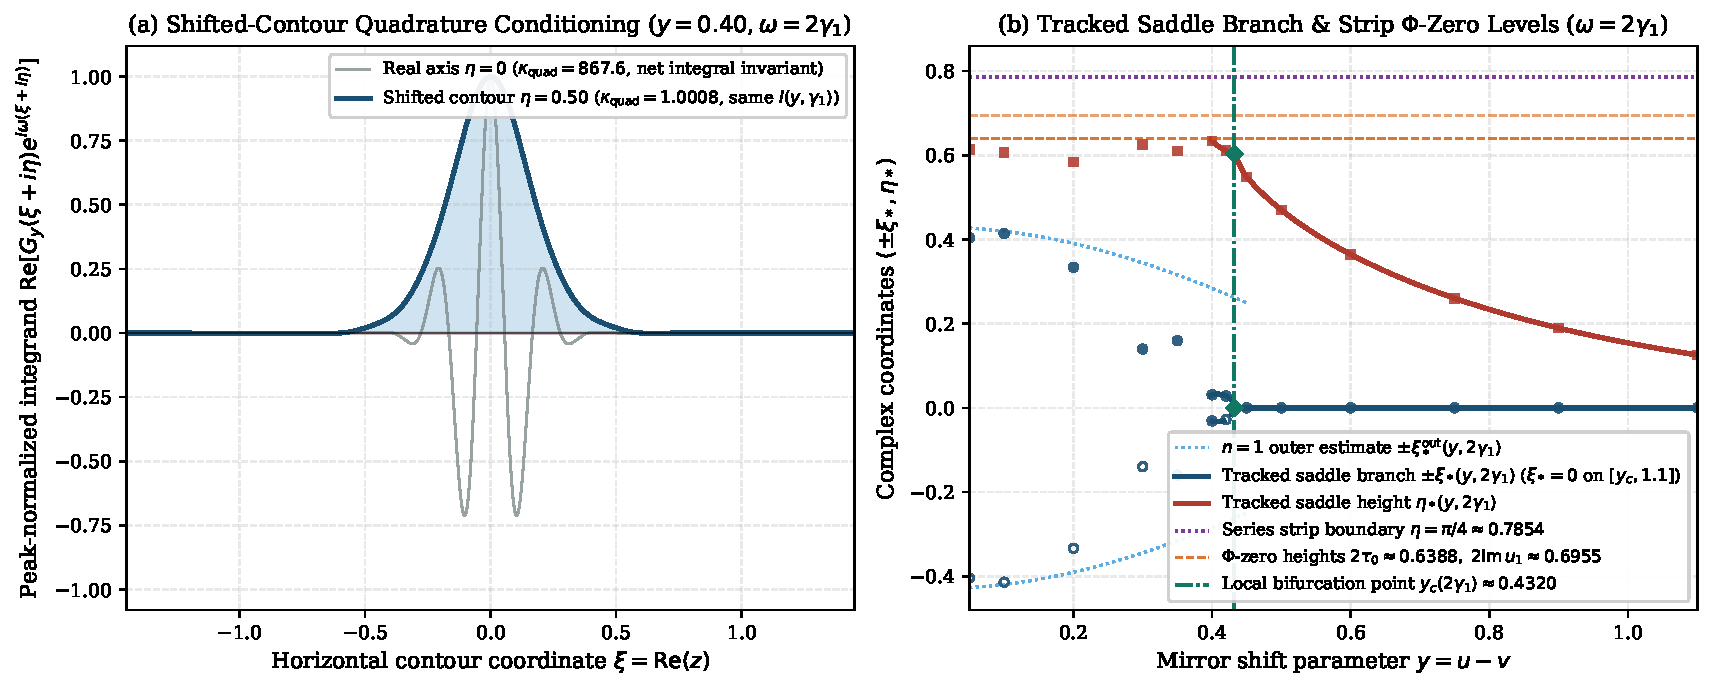
\includegraphics[width=0.98\textwidth]{figures/fig1_wigner_saddle_coalescence.pdf}
\caption{\textbf{(a)} Peak-normalized integrand $\Rea[G_y(\xi+\ii\eta)\ee^{\ii\omega(\xi+\ii\eta)}]$ at $y = 0.40$, $\omega = 2\gamma_1$: the net integral $I(y,\gamma_1) = 1.76903968\times 10^{-6}$ is contour-invariant, while shifting from $\eta = 0$ to $\eta = 0.50$ lowers the $L^1$ quadrature condition number $\kappa_{\mathrm{quad}}$ from $867.6$ to $1.0008$. \textbf{(b)} Numerically tracked stationary-point branch $(\pm\xi_*,\eta_*)$ at $\omega = 2\gamma_1$ alongside the strip $\Phi$-zero heights $2\tau_0 \approx 0.6388$ and $2\Ima(u_1) \approx 0.6955$.}\label{fig:saddle_coalescence}
\end{figure}

\subsection{Quadrature conditioning and canonical normalization verification}

At $y = 0.40$ and $\omega = 2\gamma_1$, the net integral $I(0.40,\gamma_1) = +1.76903968 \times 10^{-6}$ is invariant across $\eta \in [0, 0.60]$. Shifting from $\eta = 0$ (where $I_+ = +7.6829 \times 10^{-4}$, $I_- = -7.6653 \times 10^{-4}$, and $\kappa_{\mathrm{quad}} = 867.60$) to $\eta = 0.50$ (where $I_+ = +1.7697 \times 10^{-6}$, $I_- = -6.9457 \times 10^{-10}$, and $\kappa_{\mathrm{quad}} = 1.0008$) strongly improves numerical quadrature conditioning. Table~\ref{tab:zeros_lever} verifies both $\int_0^\infty I(y,\gamma_k)\,\dd y = 0$ and the canonical prefactor $16$ in \eqref{eq:W_mirror_thm} against direct Cauchy--Riemann evaluation $W_{\mathrm{CR}}(0.20, \gamma_k)$ to $54$--$58$ decimals across $\gamma_1, \dots, \gamma_5$.

\begin{table}[htbp]
\centering
\caption{$50$-decimal verification of the zero-marginal identity $\int_0^\infty I(y,\gamma_k)\,\dd y = 0$, canonical Wronskian normalization $W_{\mathrm{Wig}}(0.20,\gamma_k) = 16\int_0^\infty y\sinh(0.40 y)I(y,\gamma_k)\,\dd y$ versus exact $W_{\mathrm{CR}}(0.20,\gamma_k)$, and sign-change count of $I(y,\gamma_k)$ on $[0, 1.35]$.}\label{tab:zeros_lever}
\scriptsize
\setlength{\tabcolsep}{4.2pt}
\begin{tabular}{lrrrrrr}
\toprule
\textbf{Zero} & $\gamma_k$ & $\int_0^\infty I(y,\gamma_k)\,\dd y$ & $W_{\mathrm{Wig}}(0.20,\gamma_k)$ & $W_{\mathrm{CR}}(0.20,\gamma_k)$ & $|W_{\mathrm{Wig}}-W_{\mathrm{CR}}|$ & \textbf{Crossings} \\
\midrule
$\gamma_1$ & $14.134725$ & $-3.68 \times 10^{-54}$ & $+3.8445657091 \times 10^{-7}$  & $+3.8445657091 \times 10^{-7}$  & $7.07 \times 10^{-55}$ & $1$ \\
$\gamma_2$ & $21.022040$ & $+9.22 \times 10^{-55}$ & $+6.3713228683 \times 10^{-11}$ & $+6.3713228683 \times 10^{-11}$ & $9.85 \times 10^{-58}$ & $1$ \\
$\gamma_3$ & $25.010858$ & $+1.07 \times 10^{-54}$ & $+3.2438994312 \times 10^{-13}$ & $+3.2438994312 \times 10^{-13}$ & $2.09 \times 10^{-55}$ & $5$ \\
$\gamma_4$ & $30.424876$ & $-1.54 \times 10^{-53}$ & $+1.1892708589 \times 10^{-16}$ & $+1.1892708589 \times 10^{-16}$ & $2.15 \times 10^{-54}$ & $6$ \\
$\gamma_5$ & $32.935062$ & $-1.32 \times 10^{-54}$ & $+3.4236969843 \times 10^{-18}$ & $+3.4236969843 \times 10^{-18}$ & $2.45 \times 10^{-55}$ & $7$ \\
\bottomrule
\end{tabular}
\end{table}

\begin{figure}[htbp]
\centering
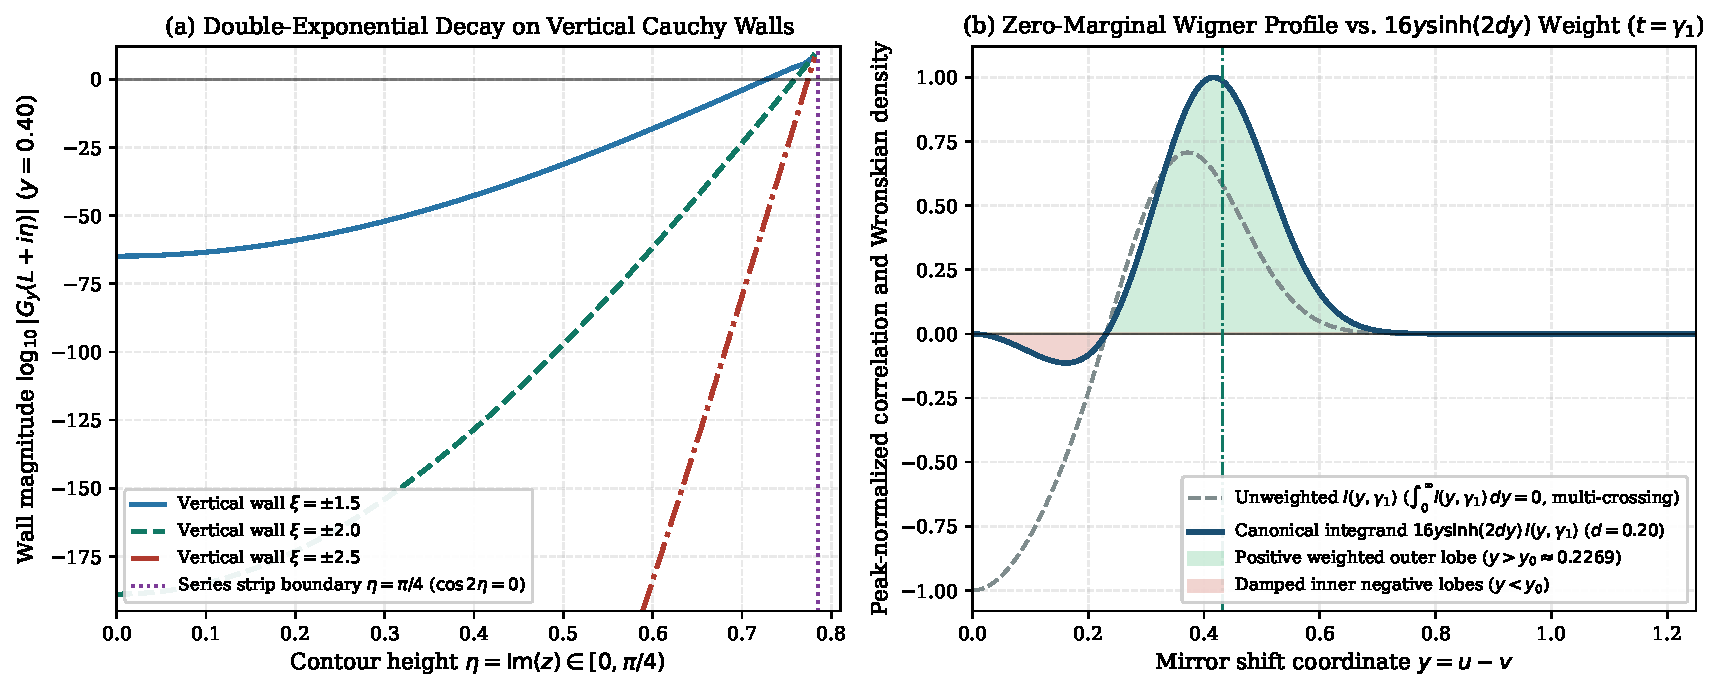
\includegraphics[width=0.98\textwidth]{figures/fig2_cauchy_contour_and_karlin_lever.pdf}
\caption{\textbf{(a)} Double-exponential decay $\log_{10}|G_y(L+\ii\eta)|$ on vertical walls $\xi = \pm L$ ($y = 0.40$) up to the series strip boundary $\eta = \pi/4$. \textbf{(b)} Unweighted zero-marginal profile $I(y,\gamma_1)$ versus the canonical weighted integrand $16 y\sinh(2d y)I(y,\gamma_1)$ at $d = 0.20$.}\label{fig:wall_and_lever}
\end{figure}

\section{Scope, limitations, and explicit obstructions}\label{sec:scope}

To delineate strictly what the phase-space and contour formalism can and cannot establish, we record four explicit obstructions:
\begin{enumerate}
\item \textbf{Contour invariance versus sign proof:} By Cauchy's theorem, \eqref{eq:shifted_I_thm} equals $I(y,t)$ identically for every $\eta \in (0,\pi/4)$. Shifting $\eta$ reduces the $L^1$ norm of the integrand (conditioning numerical quadrature), but cannot turn a negative integral positive; indeed, $I(y,\gamma_1) < 0$ for $y \in (0, 0.2269)$, where shifted contours simply exhibit negative dominant lobes.
\item \textbf{Zeros of $\Phi(u)$ and steepest-descent topology inside $\mathcal{S}_{\pi/4}$:} Because $\Phi(\ii\tau_0) = 0$ at $\tau_0 \approx 0.319415 < \pi/8$ and $\Phi(u_1) = 0$ at $u_1 \approx 0.127824 + 0.347770\ii$ ($2\tau_0 \approx 0.638830$ and $2\Ima u_1 \approx 0.695540$, both inside $\mathcal{S}_{\pi/4}$), $G_y(z)$ has zeros inside $\mathcal{S}_{\pi/4}$ creating logarithmic branch points in $\ln G_y(z)$ above $\eta_c(2\gamma_1) \approx 0.602715$ (which the tracked saddle height approaches for small $y$ and large $\omega$). While horizontal contours $z = \xi + \ii\eta$ remain valid throughout $|\eta| < \pi/4$ by holomorphy of $G_y(z)$, any global steepest-descent deformation for $\exp(\ln G_y(z) + \ii\omega z)$ across $\mathcal{S}_{\pi/4}$ must account for Stokes lines around logarithmic sinks $G_y(z_0)=0$.
\item \textbf{Multi-crossing oscillations as $t$ grows:} For $k \ge 3$, $I(y,\gamma_k)$ changes sign multiple times (Table~\ref{tab:zeros_lever}), so Karlin's single-crossing sign variation lemma does not yield $W(d,\gamma_k) > 0$.
\item \textbf{Davenport--Heilbronn and backward heat-flow obstruction:} Every identity in Proposition~\ref{prop:mirror_wigner} uses only real-evenness and rapid decay of $\Phi(u)$, never the Euler product of $\zeta(s)$. If $\Phi$ is replaced by $\Phi_\lambda(u) = \ee^{\lambda u^2}\Phi(u)$ with $\lambda < 0$ (backward de Bruijn--Newman flow $H_\lambda$ \cite{DeBruijn1950,Newman1976,CsordasNorfolkVarga1986}) or by the kernel of the Davenport--Heilbronn function \cite{DavenportHeilbronn1936,Titchmarsh1986}, then $W_\lambda(d,t) = 16\int_0^\infty y\sinh(2d y)I_\lambda(y,t)\,\dd y$ has the \emph{exact same} Wigner--$\sinh(2dy)$ form, yet $H_\lambda$ ($\lambda < 0$) and Davenport--Heilbronn possess infinitely many off-critical zeros where $W < 0$ nearby. Hence phase-space and saddle analysis of $\Phi$ alone cannot exclude off-critical zeros without arithmetic input distinguishing $\zeta(s)$ from non-Euler-product Dirichlet series.
\end{enumerate}

\appendix

\section{Heuristic single-mode $n=1$ saddle scales}\label{app:n1_scales}

Retaining only the $n=1$ term $\phi_1(u) \approx 2\pi^2\ee^{9u}\exp(-\pi\ee^{4u})$ for $u$ with large positive real part gives two heuristic comparison scales used in Figure~\ref{fig:saddle_coalescence}(b):
\begin{enumerate}
\item For $\xi > y \ge 0$, $\partial_z\ln G_y^{(1)}(z) \approx 9 - 4\pi\cosh(2y)\ee^{2z}$, so $\partial_z\ln G_y^{(1)}(z) + \ii\omega = 0$ yields $\ee^{2z_*} = \frac{9 + \ii\omega}{4\pi\cosh(2y)}$, giving $\eta_*^{\mathrm{out}}(\omega) = \frac{1}{2}\arctan(\omega/9)$ ($\approx 0.631289 < \pi/4$ at $\omega = 2\gamma_1$) and $\xi_*^{\mathrm{out}}(y,\omega) = \frac{1}{2}\ln\frac{\sqrt{\omega^2+81}}{4\pi\cosh(2y)}$.
\item In the heuristic regime $0 \le |\xi| \ll y$ where $\Phi((z-y)/2)$ varies more slowly than $\Phi((z+y)/2)$, $\partial_z\ln G_y^{(1)}(z) \approx \frac{9}{2} - 2\pi\ee^{y+z}$, giving the rough coalescence scale $y_c^{\mathrm{inner}}(\omega) \approx \frac{1}{2}\ln(\frac{\omega}{4\pi}) \approx 0.405379$ at $\omega = 2\gamma_1$ (within $6.2\%$ of the exact root $y_c(2\gamma_1) \approx 0.432021$). Because $n \ge 2$ theta modes and the subleading $-3\pi\ee^{5u}$ term are non-negligible near $u \approx 0$, these $n=1$ expressions serve purely as heuristic guides rather than asymptotic theorems at finite height.
\end{enumerate}

\section*{Use of AI and Computational Tools}

Portions of the symbolic algebra exploration, literature cross-checking, \LaTeX{} manuscript preparation, and high-precision Python/\texttt{mpmath} verification script (\nolinkurl{scripts/verify_paper1_wigner_saddle_coalescence.py}) were assisted by \textbf{Gemini} (Google DeepMind). All mathematical proofs, normalizations, counterexample checks, and numerical outputs were independently verified at $50$--$60$ decimal places.

\begin{thebibliography}{99}

\bibitem{ChesterFriedmanUrsell1957}
C.~Chester, B.~Friedman, and F.~Ursell,
\emph{An extension of the method of steepest descents},
Proc.\ Cambridge Philos.\ Soc.\ \textbf{53} (1957), 599--611.

\bibitem{CsordasNorfolkVarga1986}
G.~Csordas, T.~S.~Norfolk, and R.~S.~Varga,
\emph{The Riemann hypothesis and the Tur\'an inequalities},
Trans.\ Amer.\ Math.\ Soc.\ \textbf{296} (1986), no.~2, 521--541.

\bibitem{DavenportHeilbronn1936}
H.~Davenport and H.~Heilbronn,
\emph{On the zeros of certain Dirichlet series. I, II},
J.\ London Math.\ Soc.\ \textbf{11} (1936), 181--185, 307--312.

\bibitem{DeBruijn1950}
N.~G.~de~Bruijn,
\emph{The roots of trigonometric integrals},
Duke Math.\ J.\ \textbf{17} (1950), 197--226.

\bibitem{Hinkkanen1997}
A.~Hinkkanen,
\emph{On functions of bounded type},
Complex Variables Theory Appl.\ \textbf{34} (1997), no.~1--2, 119--139.

\bibitem{Hudson1974}
R.~L.~Hudson,
\emph{When is the Wigner quasi-probability density non-negative?},
Rep.\ Math.\ Phys.\ \textbf{6} (1974), no.~2, 249--252.

\bibitem{Karlin1968}
S.~Karlin,
\emph{Total Positivity, Vol.~I},
Stanford Univ.\ Press, Stanford, CA, 1968.

\bibitem{Lagarias1999}
J.~C.~Lagarias,
\emph{On a positivity property of the Riemann $\xi$-function},
Acta Arith.\ \textbf{89} (1999), no.~3, 217--234.

\bibitem{Newman1976}
C.~M.~Newman,
\emph{Fourier transforms with only real zeros},
Proc.\ Amer.\ Math.\ Soc.\ \textbf{61} (1976), no.~2, 245--251.

\bibitem{Olver1974}
F.~W.~J.~Olver,
\emph{Asymptotics and Special Functions},
Academic Press, New York, 1974.

\bibitem{Polya1926}
G.~P\'olya,
\emph{Bemerkung \"uber die Integraldarstellung der Riemannschen $\xi$-Funktion},
Acta Math.\ \textbf{48} (1926), 305--317.

\bibitem{Riemann1859}
B.~Riemann,
\emph{Ueber die Anzahl der Primzahlen unter einer gegebenen Gr\"osse},
Monatsber.\ K\"onigl.\ Preuss.\ Akad.\ Wiss.\ Berlin (1859), 671--680.

\bibitem{Speiser1934}
A.~Speiser,
\emph{Geometrisches zur Riemannschen Zetafunktion},
Math.\ Ann.\ \textbf{110} (1934), 514--521.

\bibitem{Titchmarsh1986}
E.~C.~Titchmarsh,
\emph{The Theory of the Riemann Zeta-Function},
2nd ed., revised by D.~R.~Heath-Brown, Oxford Univ.\ Press, Oxford, 1986.

\bibitem{Wigner1932}
E.~Wigner,
\emph{On the quantum correction for thermodynamic equilibrium},
Phys.\ Rev.\ \textbf{40} (1932), 749--759.

\end{thebibliography}

\end{document}
